%%%%%%%%%%%%%%%%%%%%%%%%%%%%%%%%%%%%%%%%%%%%%%%%%%%%%%%%%%%%%%%%%%%%%%%%%%%%%%%%
%
% Tab 1: Winner variants
%
%%%%%%%%%%%%%%%%%%%%%%%%%%%%%%%%%%%%%%%%%%%%%%%%%%%%%%%%%%%%%%%%%%%%%%%%%%%%%%%%

% full size table is table*
\begin{table*}[!tbp]
\centering
\scriptsize
\hline
\csvreader[separator=tab,
tabular=ccrrp{0.4\textwidth},
head,
table head=\bfseries Chrom. & \bfseries Cytoband & \bfseries Pos (hg38) & \bfseries Variant & \bfseries GWAS Categories\\\hline,
]{\floatRelativePath/cmpt_count_per_rsid.py/count_per_rsid_gwas_ms.tsv}{}% use head of csv as column names
{\csvcoli\ & \csvcolii\ & \csvcoliii\ & \csvcoliv & \csvcolv}% specify your coloumns here
\hline
%
\vspace{15pt}
%
  \caption{Colocalized eQTL/GWAS variants involved in 6 or more GWAS categories. Genomic coordinates are given for the hg38 assembly. }\label{tab:pleitropic_variants}
\end{table*}

%%%%%%%%%%%%%%%%%%%%%%%%%%%%%%%%%%%%%%%%%%%%%%%%%%%%%%%%%%%%%%%%%%%%%%%%%%%%%%%%%
%%
%% Fig 1: GO of pleiotropic variants
%%
%%%%%%%%%%%%%%%%%%%%%%%%%%%%%%%%%%%%%%%%%%%%%%%%%%%%%%%%%%%%%%%%%%%%%%%%%%%%%%%%%
%
%\begin{figure*}[!tbp]
%\centering
%%
%\begin{subfigure}[]{0.99\textwidth}
%\textbf{a}
%\\
%\includegraphics[width=\textwidth]{\floatRelativePath/pltbar_davidgo.py/david_pleio_3.png}
%\end{subfigure}
%
%\begin{subfigure}[]{.99\textwidth}
%\textbf{b}
%\\
%\includegraphics[width=\textwidth]{\floatRelativePath/pltbar_davidgo.py/david_pleio_2.png}
%\end{subfigure}
%%
%\caption{Gene ontology analysis of eGenes of variants associated to three (\textbf{a}) and two (\textbf{b}) GWAS categories compared to eGenes of variants associated to one GWAS category.} \label{fig:geneontology}
%\end{figure*}

%%%%%%%%%%%%%%%%%%%%%%%%%%%%%%%%%%%%%%%%%%%%%%%%%%%%%%%%%%%%%%%%%%%%%%%%%%%%%%%%%%
%%%
%%% Fig 2: Fisher stat of tissues in variants as a function of gwas category count
%%%
%%%%%%%%%%%%%%%%%%%%%%%%%%%%%%%%%%%%%%%%%%%%%%%%%%%%%%%%%%%%%%%%%%%%%%%%%%%%%%%%%%
%
%\begin{figure*}[!tbp]
%\centering
%%
%\begin{subfigure}[]{.66\textwidth}
%\textbf{a}
%\\
%\includegraphics[width=\textwidth]{\floatRelativePath/pltbar_tissue_enrich_in_pleio.py/plt.png}
%\end{subfigure}
%%
%\caption{Tissue category odds ratio in pleitropic variants compared with variant with GWAS category count 1.} \label{fig:tissues}
%\end{figure*}
%
%%%%%%%%%%%%%%%%%%%%%%%%%%%%%%%%%%%%%%%%%%%%%%%%%%%%%%%%%%%%%%%%%%%%%%%%%%%%%%%%
%
% Tab 2: Winner regions
%
%%%%%%%%%%%%%%%%%%%%%%%%%%%%%%%%%%%%%%%%%%%%%%%%%%%%%%%%%%%%%%%%%%%%%%%%%%%%%%%%

% full size table is table*
\begin{table*}[!tbp]
\centering
\scriptsize
\hline
\csvreader[
separator=tab,
tabular=ccrrp{0.45\textwidth},
head,
table head=\bfseries Chrom. & \bfseries Cytoband & \bfseries Start & \bfseries End & \bfseries GWAS Categories\\\hline,
]{\floatRelativePath/cmpt_pleiotropic_regions.py/region_window_ms_100000.tsv}{}% use head of csv as column names
{\csvcoli\ & \csvcolii\ & \csvcoliii\ & \csvcoliv & \csvcolv}% specify your coloumns here
\hline
%
\vspace{15pt}
\caption{Pleiotropic regions involving 5 or more GWAS categories. Genomic coordinates are given for the hg38 assembly.}\label{tab:pleiotropic_regions}
\end{table*}
%
%%%%%%%%%%%%%%%%%%%%%%%%%%%%%%%%%%%%%%%%%%%%%%%%%%%%%%%%%%%%%%%%%%%%%%%%%%%%%%%%%
%%
%% Fig 2: Length histogram of regions
%%
%%%%%%%%%%%%%%%%%%%%%%%%%%%%%%%%%%%%%%%%%%%%%%%%%%%%%%%%%%%%%%%%%%%%%%%%%%%%%%%%%
%
\begin{figure*}[!tbp]
\centering
%
\begin{subfigure}[]{.33\textwidth}
\textbf{a}
\\
\includegraphics[width=\textwidth]{\floatRelativePath/cmpt_pleiotropic_regions.py/regions_100000_length_hist.png}
\end{subfigure}
%
\begin{subfigure}[]{.33\textwidth}
\textbf{b}
\\
\includegraphics[width=\textwidth]{\floatRelativePath/pltbar_pleiotropic_regions_cumsum.py/pltbar_regions_cumsum.png}
\end{subfigure}
%
\caption{Analysis of pleiotropic regions. \textbf{a}, Length distribution of pleiotropic regions. \textbf{b}, Cumulative sum ordered inversely with the number of GWAS categories.} \label{fig:pleiotropy_region_distribution}
\end{figure*}
%
%%%%%%%%%%%%%%%%%%%%%%%%%%%%%%%%%%%%%%%%%%%%%%%%%%%%%%%%%%%%%%%%%%%%%%%%%%%%%%%%%
%%
%% Fig 1: Histograms variants vs GWAS, eGene and eTissues
%%
%%%%%%%%%%%%%%%%%%%%%%%%%%%%%%%%%%%%%%%%%%%%%%%%%%%%%%%%%%%%%%%%%%%%%%%%%%%%%%%%%
%
\begin{figure*}[!tbp]
\centering
%
\begin{subfigure}[]{.32\textwidth}
\textbf{a}
\\
\includegraphics[width=\textwidth]{\floatRelativePath/plthst_gwas_egene_etissue.py/hist_gwas.png}
\end{subfigure}
%
\begin{subfigure}[]{.32\textwidth}
\textbf{b}
\\
\includegraphics[width=\textwidth]{\floatRelativePath/plthst_gwas_egene_etissue.py/hist_egene.png}
\end{subfigure}
%
\begin{subfigure}[]{.32\textwidth}
\textbf{c}
\\
\includegraphics[width=\textwidth]{\floatRelativePath/plthst_gwas_egene_etissue.py/hist_etissue.png}
\end{subfigure}
%
\caption{Percentage of colocalized eQTL/GWAS variants with different number of GWAS categories (\textbf{a}), eGenes (\textbf{b}) and eTissues (\textbf{c}).} \label{fig:hist_gwas_egene_etissue}
\end{figure*}
%
%%%%%%%%%%%%%%%%%%%%%%%%%%%%%%%%%%%%%%%%%%%%%%%%%%%%%%%%%%%%%%%%%%%%%%%%%%%%%%%%%
%%
%% Fig 2: Scatter plots of winner regions
%%
%%%%%%%%%%%%%%%%%%%%%%%%%%%%%%%%%%%%%%%%%%%%%%%%%%%%%%%%%%%%%%%%%%%%%%%%%%%%%%%%%
%
%
\begin{figure*}[!tbp]

\begin{subfigure}[]{.32\textwidth}
\textbf{a}
\\
\includegraphics[width=\textwidth]{\floatRelativePath/pltsctr_x_per_rsid_y_gwas.py/count_per_rsid_chr5_start131912097_end132802472_categories9.png}
\end{subfigure}
%
\begin{subfigure}[]{.32\textwidth}
\textbf{b}
\\
\includegraphics[width=\textwidth]{\floatRelativePath/pltsctr_x_per_rsid_y_gwas.py/count_per_rsid_chr17_start39548459_end40421164_categories8.png}
\end{subfigure}
%
\begin{subfigure}[]{.32\textwidth}
\textbf{c}
\\
\includegraphics[width=\textwidth]{\floatRelativePath/pltsctr_x_per_rsid_y_gwas.py/count_per_rsid_chr17_start48116861_end49436349_categories8.png}
\end{subfigure}


\begin{subfigure}[]{.32\textwidth}
\textbf{d}
\\
\includegraphics[width=\textwidth]{\floatRelativePath/pltsctr_x_per_rsid_y_egene.py/count_per_rsid_chr5_start131912097_end132802472_categories9.png}
\end{subfigure}
%
\begin{subfigure}[]{.32\textwidth}
\textbf{e}
\\
\includegraphics[width=\textwidth]{\floatRelativePath/pltsctr_x_per_rsid_y_egene.py/count_per_rsid_chr17_start39548459_end40421164_categories8.png}
\end{subfigure}
%
\begin{subfigure}[]{.32\textwidth}
\textbf{f}
\\
\includegraphics[width=\textwidth]{\floatRelativePath/pltsctr_x_per_rsid_y_egene.py/count_per_rsid_chr17_start48116861_end49436349_categories8.png}
\end{subfigure}

\begin{subfigure}[]{.32\textwidth}
\textbf{g}
\\
\includegraphics[width=\textwidth]{\floatRelativePath/pltsctr_x_per_rsid_y_etissue.py/count_per_rsid_chr5_start131912097_end132802472_categories9.png}
\end{subfigure}
%
\begin{subfigure}[]{.32\textwidth}
\textbf{h}
\\
\includegraphics[width=\textwidth]{\floatRelativePath/pltsctr_x_per_rsid_y_etissue.py/count_per_rsid_chr17_start39548459_end40421164_categories8.png}
\end{subfigure}
%
\begin{subfigure}[]{.32\textwidth}
\textbf{i}
\\
\includegraphics[width=\textwidth]{\floatRelativePath/pltsctr_x_per_rsid_y_etissue.py/count_per_rsid_chr17_start48116861_end49436349_categories8.png}
\end{subfigure}

\caption{Count of GWAS categories (\textbf{a-c}), eGenes (\textbf{d-f}) and eTissues (\textbf{g-i}) in three pleiotropic genomic regions: \textbf{a,d,g}: 5:132,239,645-132,497,907 (5q31.1), \textbf{b,e,h}: 6:31,034,839-32,478,149 (6p21.33) and \textbf{c,g,i}: 12:111,395,984-111,645,358 (12q24.1). Genomic coordinates are given for the hg38 assembly.} \label{fig:region_gwas_egenes_tissues}
%
\end{figure*}
%
%%%%%%%%%%%%%%%%%%%%%%%%%%%%%%%%%%%%%%%%%%%%%%%%%%%%%%%%%%%%%%%%%%%%%%%%%%%%%%%%%
%%
%% Fig 3: VEP consequences
%%
%%%%%%%%%%%%%%%%%%%%%%%%%%%%%%%%%%%%%%%%%%%%%%%%%%%%%%%%%%%%%%%%%%%%%%%%%%%%%%%%%
%
\begin{figure*}[!tbp]
\centering
%
\begin{subfigure}[]{.32\textwidth}
\textbf{a}
\\
\includegraphics[width=\textwidth]{\floatRelativePath/pltbar_vep_consequence.py/upstream_gene_variant.png}
%
\end{subfigure}
%
\begin{subfigure}[]{.32\textwidth}
\textbf{b}
\\
\includegraphics[width=\textwidth]{\floatRelativePath/pltbar_vep_consequence.py/intron_variant.png}
%
\end{subfigure}
%
\begin{subfigure}[]{.32\textwidth}
\textbf{c}
\\
\includegraphics[width=\textwidth]{\floatRelativePath/pltbar_vep_consequence.py/3_prime_UTR_variant.png}
%
\end{subfigure}
%
\caption{Variant effect predictor (VEP) analysis as a function of the number of GWAS catategory number for three different consequences: \textbf{a}, Upstream gene variant, \textbf{b}, intron variant and \textbf{c}, 3' UTR variant.} \label{fig:vep_consequence}
%
\end{figure*}
%
%%%%%%%%%%%%%%%%%%%%%%%%%%%%%%%%%%%%%%%%%%%%%%%%%%%%%%%%%%%%%%%%%%%%%%%%%%%%%%%%%
%%
%% Fig 4: Violin plots. eGenes, eTissues and gwas per variants
%%
%%%%%%%%%%%%%%%%%%%%%%%%%%%%%%%%%%%%%%%%%%%%%%%%%%%%%%%%%%%%%%%%%%%%%%%%%%%%%%%%%
%
\begin{figure*}[!tbp]
\centering
%
\begin{subfigure}[]{.32\textwidth}
\textbf{a}
\\
\includegraphics[width=\textwidth]{\floatRelativePath/pltbar_x_per_variant_etissue_y_egene.py/plt.png}
\end{subfigure}
%
\begin{subfigure}[]{.32\textwidth}
\textbf{b}
\\
\includegraphics[width=\textwidth]{\floatRelativePath/pltbar_x_per_variant_egene_y_etissue.py/plt.png}
\end{subfigure}
%
\begin{subfigure}[]{.32\textwidth}
\textbf{c}
\\
\includegraphics[width=\textwidth]{\floatRelativePath/pltbar_x_per_variant_egene_etissue_y_gwas.py/plt.png}
\end{subfigure}
%
\caption{Count of eGenes per variant-tissue (\textbf{a}), eTissues per variant-eGene (\textbf{b}) and GWAS categories per variant-eGene-eTissue (\textbf{c}).} \label{fig:gwas_egene_etisue_per_variant}
%
\end{figure*}
%
%%%%%%%%%%%%%%%%%%%%%%%%%%%%%%%%%%%%%%%%%%%%%%%%%%%%%%%%%%%%%%%%%%%%%%%%%%%%%%%%%
%%
%% Fig 6: TF count per GWAS category count
%%
%%%%%%%%%%%%%%%%%%%%%%%%%%%%%%%%%%%%%%%%%%%%%%%%%%%%%%%%%%%%%%%%%%%%%%%%%%%%%%%%%

\begin{figure*}[!tbp]
\centering
%
\begin{subfigure}[]{.33\textwidth}
\textbf{a}
\\
\includegraphics[width=\textwidth]{\floatRelativePath/pltbox_x_per_rsid_y_remaptf.py/bxplt_remaptf_per_rsid_flank_50.png}
\end{subfigure}
%
\begin{subfigure}[]{.33\textwidth}
\textbf{b}
\\
\includegraphics[width=\textwidth]{\floatRelativePath/pltbar_remap_crm_gwas_categories.py/remap_crm_fisher.png}
\end{subfigure}
%
\caption{Analysis of transcription factor binding. \textbf{a}, Binding count of transcription factors in the region surrounding pleiotropic variants (Radius 50 bp) as a function of the GWAS category count. \textbf{b}, Odds ratio of cis regulatory module-annotated vs non-annotated variants.} \label{fig:freq_tf_per_variant}
%
\end{figure*}
%
%%%%%%%%%%%%%%%%%%%%%%%%%%%%%%%%%%%%%%%%%%%%%%%%%%%%%%%%%%%%%%%%%%%%%%%%%%%%%%%%%
%%
%% Fig 7: beta and log pval
%%
%%%%%%%%%%%%%%%%%%%%%%%%%%%%%%%%%%%%%%%%%%%%%%%%%%%%%%%%%%%%%%%%%%%%%%%%%%%%%%%%%
%
\begin{figure*}[!tbp]
\centering
%
\begin{subfigure}[]{.33\textwidth}
\textbf{a}
\\
\includegraphics[width=\textwidth]{\floatRelativePath/pltbar_x_per_gwas_cat_y_beta.py/eqtl_beta.png}
\end{subfigure}
%
\begin{subfigure}[]{.33\textwidth}
\textbf{b}
\\
\includegraphics[width=\textwidth]{\floatRelativePath/pltbar_x_per_gwas_cat_y_beta.py/gwas_beta.png}
\end{subfigure}

\begin{subfigure}[]{.33\textwidth}
\textbf{c}
\\
\includegraphics[width=\textwidth]{\floatRelativePath/pltbar_x_per_gwas_cat_y_logpval.py/eqtl.png}
\end{subfigure}
%
\begin{subfigure}[]{.33\textwidth}
\textbf{d}
\\
\includegraphics[width=\textwidth]{\floatRelativePath/pltbar_x_per_gwas_cat_y_logpval.py/gwas.png}
\end{subfigure}

\caption{eQTL and GWAS effect size/beta (\textbf{a,b}) and eQTL and GWAS significance/p-value (\textbf{c,d}) as a function of the GWAS category count.} \label{fig:beta_pval}
%
\end{figure*}
%
%%%%%%%%%%%%%%%%%%%%%%%%%%%%%%%%%%%%%%%%%%%%%%%%%%%%%%%%%%%%%%%%%%%%%%%%%%%%%%%%%
%%
%% Fig 7: graphical conclusions
%%
%%%%%%%%%%%%%%%%%%%%%%%%%%%%%%%%%%%%%%%%%%%%%%%%%%%%%%%%%%%%%%%%%%%%%%%%%%%%%%%%%
%
\begin{figure*}[!tbp]
\centering
%
\begin{subfigure}[]{\textwidth}

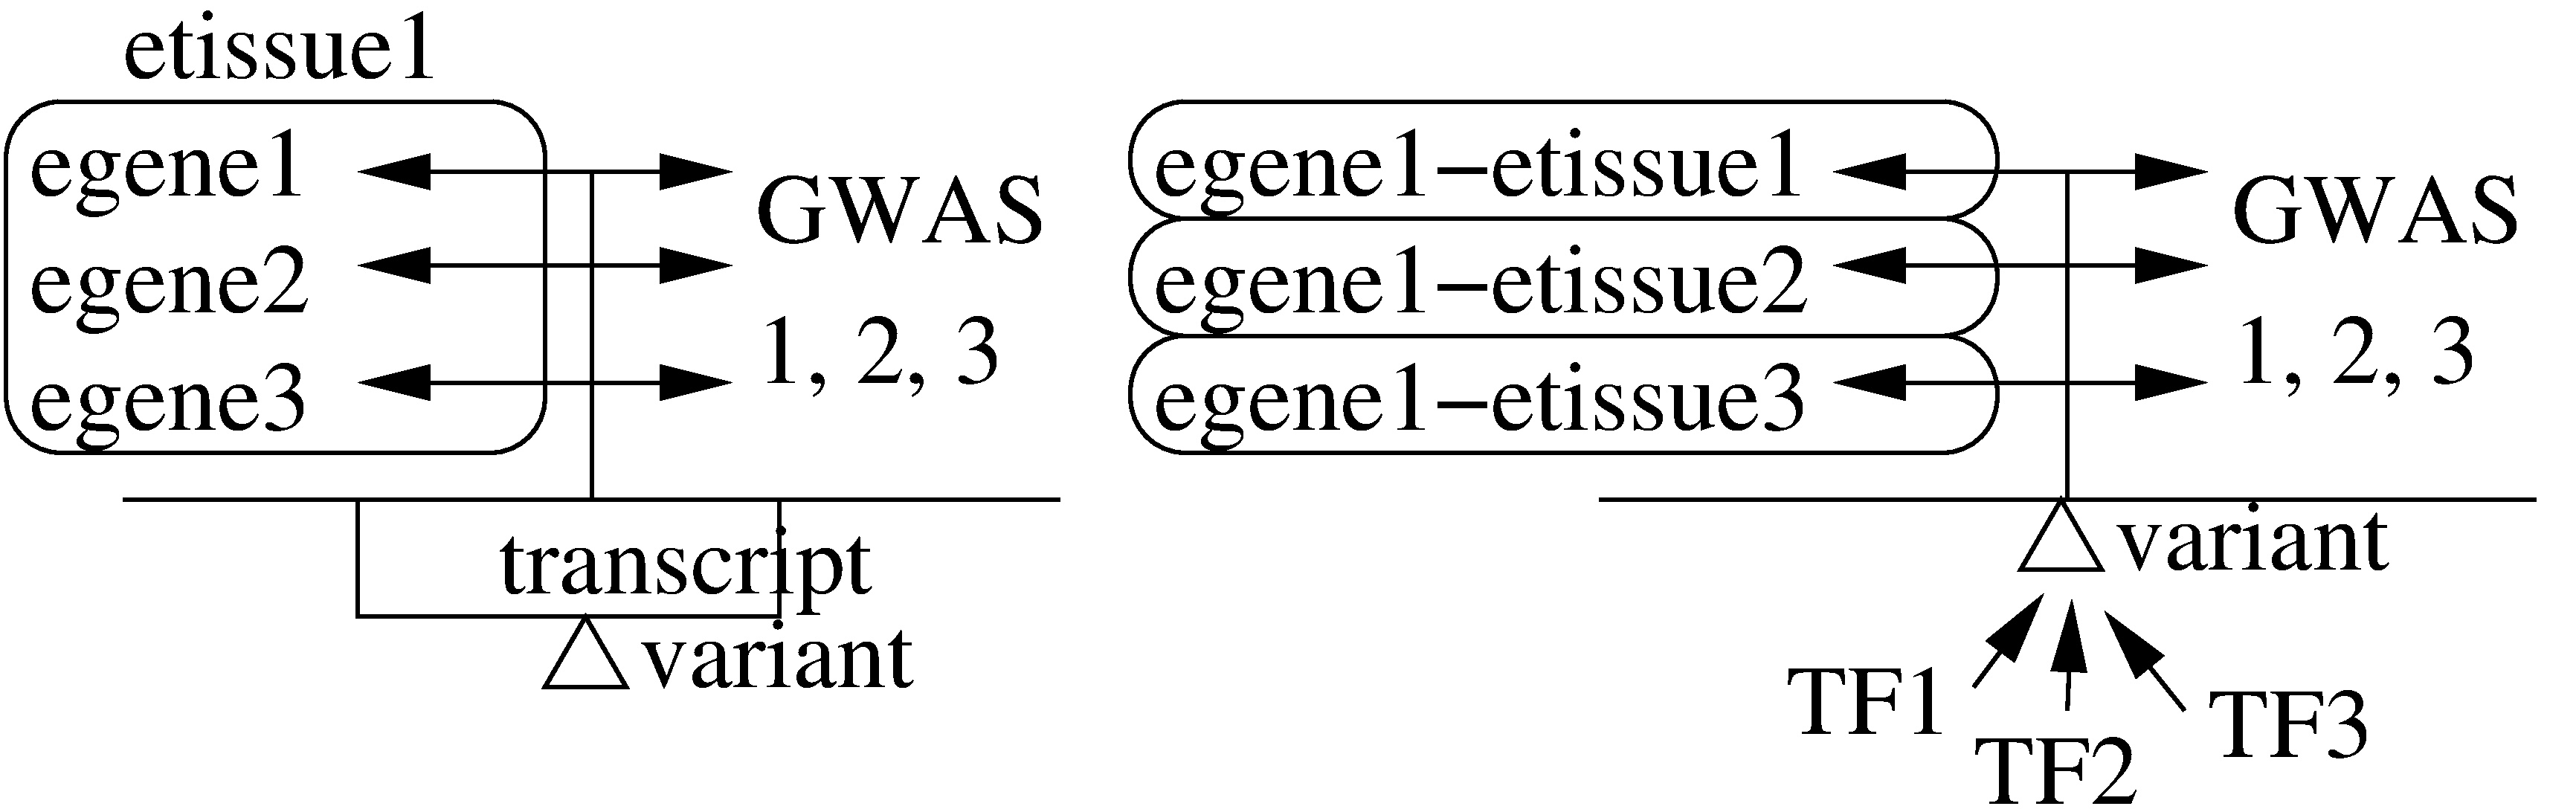
\includegraphics[width=\textwidth]{fig/graphical_summary.png}
\end{subfigure}

\caption{\textbf{Model of regulatory variant pleiotropy.} I have investigated three possible mechanisms of pleiotropy. \textbf{Left}, Pleiotropic variants have more eGenes that result in more functions and more phenotypes. This might arise from an enrichment of pleiotropic variants in splicing or 3' UTR regions. \textbf{Center}, I have also found that eGenes of pleiotropic variants are active in more etissues which result in more GWAS phenotypes. This might be explained from variants being bound by more transcription factors. \textbf{Left} Triplets of variant-eGene-eTissues are associated with more GWAS phenotypes, which directly affect the number of GWAS phenotypes. I have found that this might be explained by an enrichment of missense alleles.} \label{fig:beta}
%
\end{figure*}

